\chapter{Metodologi}

Pada bab ini penulis menjelaskan mengenai metodologi yang digunakan selama pengerjaan tugas akhir.

\begin{figure}[H]
	\begin{centering}
		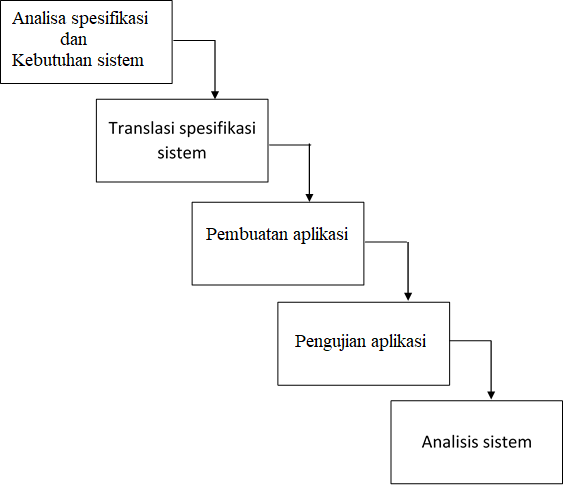
\includegraphics[scale=0.7]{metodologi_proposal}
		
		\caption{Metodologi.}
	\end{centering}
\end{figure}

\section{Analisa spesifikasi dan Kebutuhan sistem}

Menganalisa spesifikasi-spesifikasi pada teka-teki sudoku, lalu membuat kebutuhan dari aplikasi sistem yang akan mengeluarkan \textit{use case} aplikasi.

\section{Translasi spesifikasi sistem}

Aturan-aturan yang telah ditranslasikan dalam CNF di translasikan pada bahasa python dan dibuatkan aturan DIMACSnya seberti berikut:

\begin{enumerate}
	\item Setiap baris memuat bilangan antara 1 
	hingga 9 : 
	
	$\bigwedge_{r=1}^{9}$$\bigwedge_{n=1}^{9}$$\bigvee_{c=1}^{9}$$p\left(r,c,n\right)$
	
	\vspace{5mm}
	
	Skrip python :
	
	\vspace{5mm}
	
	\texttt{def aturan1(dimacs):}
	
	\qquad\qquad\texttt{for r in range(1, 10):}
	
	\qquad\qquad\qquad\texttt{for n in range(1, 10):}
	
	\qquad\qquad\qquad\qquad\texttt{for c in range(1, 10):}
	
	\qquad\qquad\qquad\qquad\qquad\texttt{dimacs += str(r) + str(c) + str(n) + ' 0\textbackslash n'}
	
	\qquad\qquad\qquad\qquad\texttt{global klausa}
	
	\qquad\qquad\qquad\qquad\texttt{klausa += 1}
	
	\qquad\qquad\texttt{return dimacs}
	
	
	\item Setiap kolom memuat bilangan antara 1 hingga 9 : 
	
	$\bigwedge_{c=1}^{9}$$\bigwedge_{n=1}^{9}$$\bigvee_{r=1}^{9}$$p\left(r,c,n\right)$
	
	
	\vspace{5mm}
	
	Skrip python :
	
	\vspace{5mm}
	
	\texttt{def aturan1(dimacs):}
	
	\qquad \qquad\texttt{for c in range(1, 10):}
	
	\qquad \qquad \qquad\texttt{for n in range(1, 10):}
	
	\qquad \qquad \qquad \qquad\texttt{for r in range(1, 10):}
	
	\qquad\qquad\qquad\qquad\qquad\texttt{dimacs += str(r) + str(c) + str(n) + ' 0\textbackslash n'}
	
	\qquad \qquad \qquad \qquad\texttt{global klausa}
	
	\qquad \qquad \qquad \qquad\texttt{klausa += 1}
	
	\qquad \qquad\texttt{return dimacs}
	
	\item Setiap submatriks atau blok $3 \times 3$
	memuat bilangan antara 1 hingga 9 : 
	
	$\bigwedge_{i=0}^{2}$$\bigwedge_{j=0}^{2}$$\bigwedge_{n=1}^{9}$$\bigvee_{r=3i+1}^{3i+3}$$\bigvee_{c=3j+1}^{3j+3}$$p\left(r,c,n\right)$
	
	
	\vspace{5mm}
	
	Skrip python :
	
	\vspace{5mm}
	
	\texttt{def aturan1(dimacs):}
	
	\qquad \qquad\texttt{for i in range(0, 3):}
	
	\qquad \qquad \qquad\texttt{for j in range(0, 3):}
	
	\qquad \qquad \qquad \qquad\texttt{for n in range(1, 10):}
	
	\qquad\qquad\qquad\qquad\qquad\texttt{for r in range(3*i+1, 3*i+4):}
	
	\qquad\qquad\qquad\qquad\qquad\qquad\texttt{for c in range(3*j+1, 3*j+4):}
	
	\qquad\qquad\qquad\qquad\qquad\qquad\qquad\texttt{dimacs += str(r) + str(c) + str(n) + ' 0\textbackslash n'}
	
	\qquad\qquad\qquad\qquad\qquad\qquad\texttt{global klausa}
	
	\qquad\qquad\qquad\qquad\qquad\qquad\texttt{klausa += 1}
	
	\qquad\qquad\texttt{return dimacs}
	
	\vspace{5mm}
	
	Setiap sel memuat paling banyak satu bilangan antara 1 hingga 9 : 
	
	\vspace{5mm}
	
	
	\item Setiap sel memuat paling banyak satu bilangan antara 1 hingga 9 : 
	
	$\bigwedge_{r=1}^{9}$$\bigwedge_{c=1}^{9}$$\bigwedge_{n=1}^{8}$$\bigwedge_{i=n+1}^{9}$
	$\left(\neg p\left(r,c,n\right)\vee\neg p\left(r,c,i\right)\right)$
	
	
	\vspace{5mm}
	
	Skrip python :
	
	\vspace{5mm}
	
	\texttt{def aturan1(dimacs):}
	
	\qquad \qquad\texttt{for e in range(0, 3):}
	
	\qquad \qquad \qquad\texttt{for c in range(0, 3):}
	
	\qquad \qquad \qquad \qquad\texttt{for n in range(1, 9):}
	
	\qquad\qquad\qquad\qquad\qquad\texttt{for i in range(n+1, 10):}
	
	\qquad\qquad\qquad\qquad\qquad\qquad\texttt{dimacs += '-' + str(r) + str(c) + str(n) + ' ' + '-' + str(r) + str(c) + str(i) + ' 0\textbackslash n'}
	
	\qquad\qquad\qquad\qquad\qquad\texttt{global klausa}
	
	\qquad\qquad\qquad\qquad\qquad\texttt{klausa += 1}
	
	\qquad \qquad\texttt{return dimacs}
	
\end{enumerate}

\section{Pembuatan aplikasi}

Spesifikasi yang sudah dalam bentuk CNF akan digunakan pada \textit{SAT Solver}. Lalu \textit{use case} yang didapat akan dibuat fungsionalitasnya. Pembuatan aplikasi menggunakan \textit{waterfall design} tahapan-nya berupa:

\subsection{Spesifikasi Aplikasi}

Spesifikai aplikasi adalah sebagai berikut:
\begin{enumerate}
	\item Bermain sudoku.
	\item Membuat sudoku.
	\item Memecahkan sudoku.
\end{enumerate}

\begin{figure}[H]
	\begin{centering}
		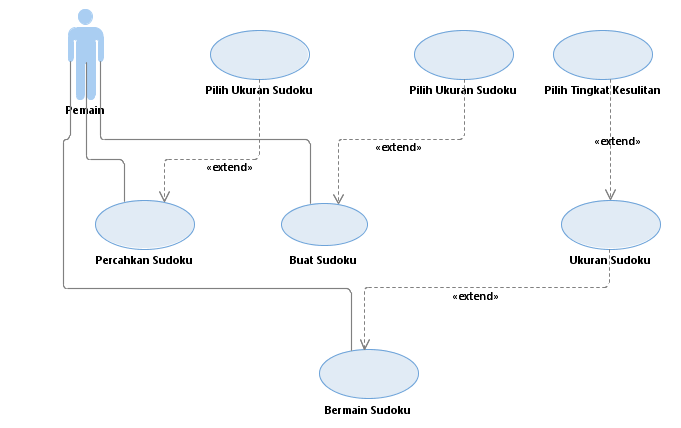
\includegraphics[scale=1]{gambar/useCase}
		
		\caption{\textit{Use Case Diagram}.}
	\end{centering}
\end{figure}

\subsection{\textit{Analysis}}

Dalam \textit{analysis}, penulis menjabarkan mulai dari hal
mendasar yaitu kendala global dalam pengembangan perangkat lunak yang sudah ada. Adapun masalahnya adalah minimnya aplikasi pemecah sudoku yang interaktif.

\subsection{\textit{Design}}

Fitur yang akan ada pada aplikasi tersebut adalah sebagai berikut

 \begin{enumerate}
 	\item Bermain sudoku.
 	\item Membuat sudoku.
 	\item Pecahkan sudoku.
 \end{enumerate}

\subsection{Implementasi}

Lalu dalam tahap \textit{coding} penulis akan menggunakan
bahasa pemograman python dengan SAT \textit{solver} \cite{SATPy2} sebagai dasarnya. Setelah itu akan ditambahkan GUI dan \textit{use case} yang telah di buat.

\section{Pengujian aplikasi}

Pada tahap ini aplikasi akan diujikan kebeberapa penguji dengan diberikan lembat \textit{test case} yang meliputi beberapa aspek kualitas pada aplikasi. Teknik yang digunakan pada pengujian adalah pengujian kotak hitam \cite{TEST1}.

\section{Analisis sistem}

Menganalisa kelayakan kualitas dari aplikasi berdasarkan hasil dari pengujian.